\chapter{Analysis Overview}\label{sec:analysis_overview}

\section{History of the \hzg{} Search}
Both the CMS and ATLAS collaborations have undertaken the search for \hzg{} since Run 1 of the LHC. 
Before the CMS Run 2 analysis, which is the focus of this thesis, each collaboration published results using 
Run 1 data at $\sqrt s = 7$ and 8\TeV~\cite{cms-HZG,atl-HZG}, CMS published a result with 2016 data at $\sqrt s = 13\TeV$~\cite{Sirunyan:2018tbk}, and 
ATLAS published a full Run 2 result at $\sqrt s = 13\TeV$~\cite{Aad:2020plj}. As such, the present analysis represents the continuation 
of a broader effort, so we will give a brief history of these prior searches to put our work in context. While 
some of the analysis strategies of past searches inform our current strategy, there are also many differences 
and innovations in our analysis. We will emphasize the ways in which our analysis 
overlaps and differs with previous approaches, and will show that our innovations have significantly 
improved the expected sensitivity and statistical robustness of the search. 

\subsection{The Run 1 Searches}
In 2014, ATLAS published its Run 1 results~\cite{atl-HZG} for the search for \hzg{} where $\mathrm{Z}\to\ell^+\ell^-$ with $\ell=\mathrm{e}$ or $\mu$. The baseline strategy was a standard dilepton 
plus photon selection, with $m_{\ell^+\ell^-}$ near the Z boson mass and $\ell^+\ell^-\gamma$ invariant mass ($m_{\ell^{+}\ell^{-}\gamma}$) between 115 and 170\GeV. The resolution of $m_{\ell^{+}\ell^{-}\gamma}$ was improved using a kinematic fit procedure, accounting for the true Z boson line shape. Events were categorized based on lepton flavor; the pseudorapidity difference between the photon and Z boson; and the variable $p_{\mathrm{T}}^{t}$, defined as $\abs{\vec{p}_\mathrm{T}^{\,\PZ\gamma}\times\hat{t}}$, where $\hat{t}=(\vec{p}_\mathrm{T}^{\,Z}-\vec{p}_\mathrm{T}^{\,\gamma})/\abs{\vec{p}_\mathrm{T}^{\,Z}-\vec{p}_\mathrm{T}^{\,\gamma}}$~\cite{Ackerstaffetal.1998,VESTERINEN2009432}, the $\pt$ of the $\PZ\gamma$ system that is perpendicular to the difference of the three-momenta of the $\PZ$ boson and the photon, a quantity that is strongly correlated with the \pt of the $\lplm\gamma$ system. Limits on the signal strength relative to the SM prediction, shown in Fig. \ref{fig:run1_limits} (left), were obtained from a simultaneous fit to the $m_{\ell^{+}\ell^{-}\gamma}$ distributions in all categories.

The CMS Run 1 analysis~\cite{cms-HZG} was published in 2015. 

\begin{figure}[tb]
  \centering
   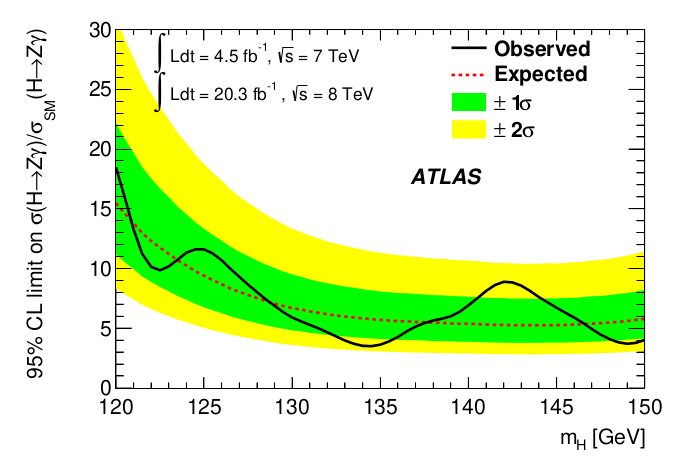
\includegraphics[width=0.45\textwidth,height=0.33\textwidth]{fig/overview/atl_run1_lim.png}
   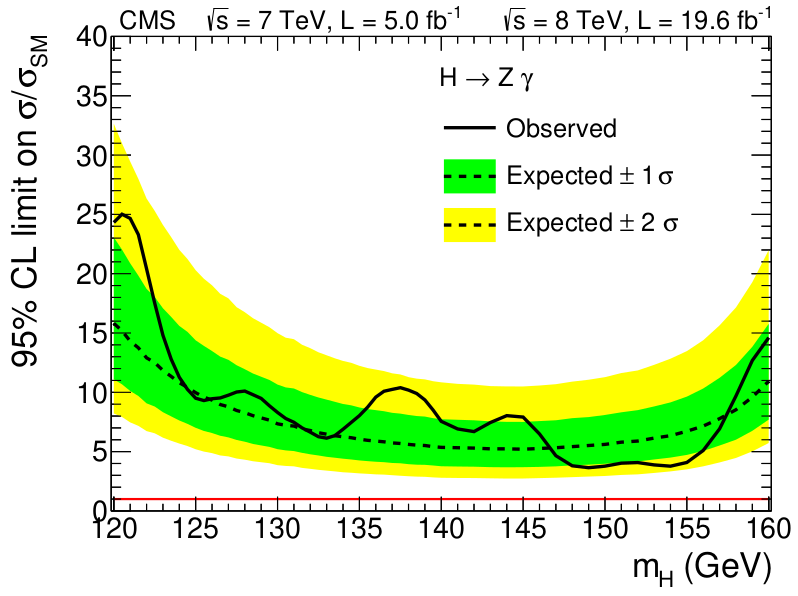
\includegraphics[width=0.45\textwidth,height=0.33\textwidth]{fig/overview/cms_run1_lim.png}
	\caption
	[ATLAS (left) and CMS (right) Run 1 limit results as a function of $m_\PH$.]
	{ATLAS (left~\cite{atl-HZG}) and CMS (right~\cite{cms-HZG}) Run 1 limit results as a function of $m_\PH$.}
	\label{fig:run1_limits}
\end{figure}


\subsection{The Previous Run 2 Searches}

\section{The CMS Run 2 Strategy}


Before discussing the full details of the analysis procedure and results, it is worth summarizing 
the broader strategy taken in our search for \hzg. As two prior CMS results have 
been published with Run 1 data and 2016 data, we will emphasize the ways in which our analysis
overlaps and differs from these previous approaches. Very broadly, the current search is 
similar to the previous analyses in trigger, object, and basic event selection. 
However, it is significantly more advanced in three body mass reconstruction, 
event categorization, and background modeling. We will show that the innovations in these 
areas have significantly improved the expected sensitivity and statistical robustness of the search 
with respect to the past CMS analyses.

Chapter 5 provides a detailed description of the data and Monte Carlo simulation 
used in our analysis. Standard dimuon and dielectron trigger streams are used for 2016, 2017, 
and 2018 LHC data. The full dataset corresponds to an integrated luminosity of 
137 $fb^{-1}$. In other words, we use the full CMS Run 2 dataset at 13 TeV center of 
mass energy. Simulated signal samples are used to determine the expected signal yields 
and three body mass shape. Simulated background samples are used for MVA training 
and category optimization. However, the background shape and normalization in the final result
is determined by fitting the data and does not rely on any simulation.

Chapter 6 describes the basic object and event selection used in the analysis, and Chapter 7 
describes further selection and categorization using MVAs. As mentioned, the basic 
selection requirements are fairly similar to previous CMS analyses. Muons are selected with 
a loose cut-based ID, while electrons and photons are selected with loose MVA IDs. Loose ID
requirements are chosen in order to maximize signal efficiency. Background is then suppressed 
through a combination of basic cuts and MVA methods. Basic kinematic cuts on isolation, mass, 
and photon energy variables are able to significantly reduce backgrounds from initial and final 
state radiation, while the MVA methods are able to strongly disciminate against backgrounds from 
jets misreconstructed as photons. Finally, a kinematic fit procedure in the dilepton mass 
is able to significantly improve the signal mass resolution. The kinematic fit is an 
innovation of the current analysis and contributes to its improved sensitivity.

Chapter 8 details the approach to signal and background modeling of the three body 
mass spectrum. As in previous CMS \hzg searches, the 
signal shape is determined via an analytic fit to simulation. A resonant background 
contribution from \hmumu is modeled similarly. The nonresonant 
background contribution is taken from a fit to data in the range of 105 to 170 GeV. This 
background model includes both the turn-on arising from the real Z boson peak as well as 
the falling spectrum at higher mass. We note that the turn-on was fit in the Run 1 analysis as 
well, but was dropped in the 2016 analysis. A more thorough discussion of the merits of fitting 
the turn-on will be described in chapter 8.

Chapter 9 describes the systematic uncertainties relevant for the analysis, and Chapter 10
gives a basic overview of the statistics used to arrive at the final results. It is 
worth noting that given the current integrated luminosity, the analysis is dominated by 
statistical uncertainty. Chapter 11 gives the full set of results, including best fit 
signal strength, limits, and comparisons with \hgg. 


